\chapter{Metodologia}
\label{cap:metodologia}

%TODO revisar
Este capítulo apresenta a metodologia adotada neste trabalho. A seção \ref{cap:metodologia:sec:conjunto_dados:sec:escolha_conjunto} descreve o processo de escolha de hotéis; a seção \ref{cap:metodologia:sec:conjunto_dados:sec:coleta_review} descreve como foi realizada a coleta das avaliações, \ref{cap:metodologia:sec:conjunto_dados:sec:pre_processamento} descreve o preparo e escolha das avaliações pós coleta.
% ; a seção \ref{subsec:pre_processamento} descreve // TODO; a seção \ref{subsec:analise_sentimentos} descreve // TODO; a seção \ref{subsec:analise_temporal} descreve // TODO

\section{Conjunto de Dados}
\label{cap:metodologia:sec:conjunto_dados}

\subsection{Escolha do conjunto}
\label{cap:metodologia:sec:conjunto_dados:sec:escolha_conjunto}

O conjunto de dados foi selecionado considerando os hotéis localizados em todo o território brasileiro e com informações disponíveis no Google Maps.

% https://developers.google.com/maps/apis-by-platform?hl=pt-br#web_service_apis
A primeira etapa consiste em identificar os hotéis distribuídos no território brasileiro por estado que estão na plataforma do Google Maps, essa tarefa é automatizada por meio da utilização do serviço exposto do Google Maps, a iteração foi realizada utilizando a biblioteca oficial do Google Maps versão escrita em Java e que está disponível publicamente no repositório \citeonline{javaGoogleMapsService2022}.

Para identificar os diversos hotéis, foi escrito um \emph{script} Kotlin \citeonline{scriptKotlinBuscarHoteis} que interage com a biblioteca supracitada para realizar a busca da lista de hotéis de forma automatizada, realizando buscas de forma sequencial considerando todos os estados brasileiros e persistindo os dados obtidos.

O objetivo nesta etapa é identificar o maior número possível de hotéis que estão disponíveis para consulta na plataforma e em posse destes obter informações mais detalhadas, como quantidade de avaliações, nota atual, localização do estabelecimento, para cada hotel para que seja possivel em posse dessa lista então realizar escolha dos hotéis para estudo.

Para essa tarefa utilizaremos a interface de \emph{Text Search Query}, informações como o nome do hotel, localização e identificador do hotel na plataforma são disponibilizadas por essa interface. Nessa interface conseguimos realizar a busca passando informações que servirão para limitar a busca, como idioma de interesse, coordenadas e diâmetro limite para ser considerado e dessa forma obter uma busca com viés dos parâmetros fornecidos \cite{placesSearchText2023}.

\lstinputlisting[language=java,caption=Fragmento de código da interface Google Maps \emph{Text Search Query}]{extras/code/googlemaps-place-search.kt}

O texto utilizado para a busca dos hotéis é definida no seguinte modelo “frase + região”. Por exemplo, na frase “hotéis próximos ao Cristo Redentor”, a API deverá retornar informações básicas de hotéis cadastrados na plataforma próximos à região do Cristo Redentor. As regiões utilizadas foram os estados e capitais brasileiros.

Após obter a lista com as informações básicas se faz necessário obter informações mais detalhadas dos estabelecimentos, para isso utilizaremos a interface de \emph{Place Details} para poder obter essas informações na plataforma, dentre as informações expostas por esta interface apenas algumas são de nosso interesse e serão utilizadas como por exemplo, mas não se restringindo à, número de avaliações disponíveis, classificação atual na plataforma e quantidade de avaliações, essas serão informações importantes no momento de escolha dos hotéis que serão utilizados no estudo, essas e outras são obtidas nessa etapa. Infelizmente por limitação da plataforma essa interface apenas lista 5 avaliaçoes aleatorias, tornado inviavel a sua utilização para coleta de grande número de avaliações, a coleta das avaliações é descrita em \ref{cap:metodologia:sec:conjunto_dados:sec:coleta_review}.

\lstinputlisting[language=java,caption=Fragmento de código da interface Google Maps \emph{Place Details}]{extras/code/googlemaps-place-details.kt}

Foi possível identificar 814 hotéis distribuídos em todo o território nacional, lista disponivel no apêndice \ref{apendice:lista_completa_hoteis}, desde hotéis de grandes redes e com disponibilidade de reservas do tipo \emph{All Inclusive} até hotéis pouco conhecidos com menos de 10 avaliações na plataforma.

Dessa lista temos como destaque os seguintes números:

Estados com a maior quantidade de hotéis
\begin{itemize}
	\item RJ: 71
	\item SP: 67
	\item PA: 62
	\item MG: 61
	\item RR/PI/MS: 60
\end{itemize}

Estados com a maior quantidade de avaliações

\begin{itemize}
	\item RJ: 231947 (4,22 com 71 hotéis)
	\item SP: 169586 (4,21 com 67 hotéis)
	\item BA: 107716 (4,34 com 22 hotéis)
	\item MG: 107067 (4,35 com 61 hotéis)
	\item PB: 68188 (4,36 com 54 hotéis)
\end{itemize}


Média da classificação dos hotéis por Estado

\begin{itemize}
	\item RS: 4,70 com 9493 avaliações no total (2 hotéis)
	\item AL: 4,64 com 33345 avaliações no total (8 hotéis)
	\item AC: 4,60 com 1696 avaliações no total (1 hotel)
	\item AM: 4,53 com 45509 avaliações no total (46 hotéis)
	\item SC: 4,50 com 32621 avaliações no total (7 hotéis)
\end{itemize}

Por conta da grande variedade de hotéis, o critério de escolha foi limitar a hotéis com disponibilidade de pacote \emph{All Inclusive} e na região nordeste, com o primeiro critério definido temos então uma lista com um grupo de 15 hotéis dentre os disponíveis após o filtro da região temos então 11.

Também foram adicionados manualmente a lista outros hotéis não foram listados nas consultas à API porém que estavam indicados na lista de regiões das principais atrações do Brasil segundo~\cite{googleFlights2022destinos}. Essa lista é composta com base nas análises conduzidas pelo Google, que considera a quantidade de menções online e as suas avaliações recebidas na plataforma. 2 novos hotéis foram adicionados e atendiam os critérios já definidos e foram adicionados à nossa lista.

Posteriormente essa lista irá servir como entrada para um \emph{Web Scraping} para buscar as avaliações onlines disponíveis no Google Maps, realizadas pelos usuários e os \emph{Local Guides}~\cite{google2022localguides} registrados na plataforma. Os detalhes da escolha das avaliações são discutidos em \ref{cap:metodologia:sec:conjunto_dados:sec:pre_processamento}.

A lista composta de 13 hotéis todos localizados na região nordeste do brasil e com a disponibilidade de pacotes \emph{All Inclusive}, no momento de consulta na plataforma do Google Maps, é valido notar que todos os hotéis da lista no momento da escolha possuíam uma avaliação na plataforma do Google Maps com nota superior a 4.20 e são todos hotéis de 4 ou 5 estrelas.

A lista de hotéis obtida é composta conforme a tabela~\ref{table:lista_hoteis}.

\begin{table}[]
	\begin{tabular}{|p{5cm}|l|r|r|l|r|}
		\hline
		\textbf{Nome}                                 & \textbf{Estado} & \textbf{Nota} & \textbf{Estrelas} & \textbf{Região} & \textbf{Quantidade} \\\hline

		Cana Brava All Inclusive Resort               & BA              & 4.60          & 4                 & NORDESTE        & 10987               \\\hline
		Grand Oca Maragogi                            & AL              & 4.30          & 5                 & NORDESTE        & 4613                \\\hline
		Hotel Marsol Beach Resort                     & RN              & 4.20          & 4                 & NORDESTE        & 3269                \\\hline
		Hotel Vila Galé - Touros                      & RN              & 4.60          & 5                 & NORDESTE        & 5619                \\\hline
		Hotel Vila Galé - Marés                       & BA              & 4.50          & 5                 & NORDESTE        & 8516                \\\hline
		Hotel Vila Galé: Eco Resort - Cabo            & PE              & 4.50          & 5                 & NORDESTE        & 5370                \\\hline
		Iberostar Bahia                               & BA              & 4.70          & 5                 & NORDESTE        & 16109               \\\hline
		La Torre Resort All Inclusive                 & BA              & 4.70          & 4                 & NORDESTE        & 6140                \\\hline
		Makai Resort Aracaju - All Inclusive          & SE              & 4.30          & 4                 & NORDESTE        & 5276                \\\hline
		Nauticomar Resort All Inclusive \& Beach Club & BA              & 4.30          & 4                 & NORDESTE        & 4258                \\\hline
		Salinas Maceió All Inclusive Resort           & AL              & 4.70          & 4                 & NORDESTE        & 4663                \\\hline
		Salinas Maragogi All Inclusive Resort         & AL              & 4.80          & 5                 & NORDESTE        & 7111                \\\hline
		Transamerica Comandatuba                      & BA              & 4.80          & 4                 & NORDESTE        & 3179                \\\hline
	\end{tabular}%
	\caption{Lista de hotéis e número de avalições}
	\label{table:lista_hoteis}
\end{table}

\subsection{Coleta das avaliações}
\label{cap:metodologia:sec:conjunto_dados:sec:coleta_review}

Já existe um \emph{script} escrito em Python \cite{gaspa93scrapper2023} que dado uma \emph{URL} do Google Maps, utilizando Selenium, obtém um determinado número de avaliações, o \emph{script} porém estava defasado e pendente de atualização, um dos \emph{forks} existentes \citeonline{ryuuzakescrapper2023} estava também pouco mais atualizado, porém ainda não funcional.


%TODO essas referencias de selenium numpy etc estão certas?
Utilizando esses projetos como base fiz um novo \emph{fork} e então atualizei o \emph{script} para realizar o trabalho de obter as avaliações dos hotéis, o \emph{script} escrito em Python e as suas principais dependências eram de \cite{selenium2023}, \citeonline{harris2020array}, \citeonline{jeffreback20226702671} e \citeonline{richardson2007beautiful}. Utilizando \citeonline{merkel2014docker} para executar o \emph{script} era possível executa-lo de forma concorrente, utilizando o Selenium e executando diversos drivers do Google Chrome, porém para esse tipo de tarefa o Selenium não é uma ferramenta eficiente e seu desempenho não é rápido, existem diferentes impactos por conta de sua utilização, os quais não serão discutidos aqui, a busca das avaliações para apenas um hotel demorava aproximadamente 3h para executar e o sucesso da execução do \emph{script} com a utilização do Selenium depende diretamente da imutabilidade da interface visual do Google Maps, o que torna esse formato não escalável dado a velocidade com que a interface do Google Maps recebe atualizações. Durante a adaptação do \emph{script} para conseguir extrair corretamente as avaliações foram realizadas 10 tentativas de execução, no período de 09/2022 à 11/2022, com periodicidade aproximadamente semanal e aproximadamente a cada duas semanas a estrutura do Google Maps mudava, estrutura essa que é parte fundamental para que a execução obtivesse sucesso, e dessa forma o \emph{script} precisava passar por nova atualização para que a nova estrutura fosse de conhecimento, existiam inclusive alguns testes no formato A/B onde alguns estabelecimentos possuiam estrutura da página do Google Maps diferente de outros, aumentando ainda mais a complexidade de manter o \emph{script} funcional.

O \emph{script} possui uma dependência muito forte com a parte estrutural da página e dessa forma qualquer mudança em \emph{tags HTML} e/ou as classes \emph{CSS} da página dos estabelecimentos no Google Maps, características de um \emph{WebScrapper}, que dificulta a manutenção e limita a sua capacidade de reutilização.

% https://github.com/emerson-matos/maps-reviews-api-scraper
Baseado no \emph{script} do \emph{WebScrapper} existe um repositório que utiliza diretamente uma API do Google chamada reviewDialog, sem a necessidade de utilizar o Selenium, que era em grande parte responsável pela baixa performance, dessa forma a coleta das avaliações ocorre de forma bem mais rápida, e em um período de aproximadamente 1h foi possível obter um total de 86.291 avaliações dos hotéis da lista.

\subsection{Pré-processamento}
\label{cap:metodologia:sec:conjunto_dados:sec:pre_processamento}

Após possuir as avaliações precisamos realizar alguns filtros para que a analise de sentimentos consiga resultar em algo concreto, dessa forma foram definidos critérios de filtro para ter uma lista final com as avaliações a serem levadas em consideração na analise.

O primeiro critério é que a avaliação precisa possuir conteúdo textual e este por sua vez precisa então possuir 3 ou mais caracteres. Como podemos observar na tabela anterior temos uma discrepancia no número de avaliações perceptível com divisão no período de 2017/2018, então apenas levaremos em consideração avaliações realizadas em 2018 ou posteriores a essa data e o ultimo critério a ser levado em consideração é que a avaliação precisa estar escrita no idioma português, e não ter sido traduzida pelo Google.

\lstinputlisting[language=Python,caption=Filtros aplicados ao dataset de avalições]{extras/code/review_filter.py}

Considerando todas as avaliações obtidas, temos:

\begin{itemize}
	\item 80470(93.25\%) enviadas depois de 2017 e 5821(6.75\%) enviadas em 2017 ou antes
	\item 56893(65.93\%) com texto e 3 ou mais caracteres, 29386(34.05\%) sem texto e 12(0.01\%) avaliações com 1 ou 2 caracteres
	\item 4184(4.85\%) avaliações traduzidas
\end{itemize}

E dentre todas as avaliações obtidas utilizaremos para a analise o total de 49219(57.04\%) e 37072(42.96\%) foram ignoradas. Assim as avaliações que foram consideradas estão então distribuídas conforme \ref{table:distribuicao_review_per_year}.


\begin{table}[]
	\centering
	\begin{tabular}{|l|l|}
		\textbf{Ano} & \textbf{Quantidade} \\\hline
		2023         & 11925               \\
		2022         & 16364               \\
		2021         & 8104                \\
		2020         & 12489               \\
		2019         & 18963               \\
		2018         & 12625               \\
		2017         & 4426                \\
		2016         & 940                 \\
		2015         & 247                 \\
		2014         & 106                 \\
		2013         & 88                  \\
		2011         & 5                   \\
		2012         & 9
	\end{tabular}%
	\caption{Quantidade de avaliações obtidas por ano}
	\label{table:review_per_year}
\end{table}

\begin{table}[]
	\centering
	\begin{tabular}{|c|crrrrr|}
		\hline
		\multicolumn{1}{|c|}{\multirow{2}{*}{\textbf{Estado}}} &
		\multicolumn{2}{c|}{\textbf{analisar}}                 &
		\multicolumn{3}{c|}{\textbf{nota}}                     &
		\multicolumn{1}{c|}{\textbf{estrelas}}                                                                            \\ \cline{2-7}
		\multicolumn{1}{|l|}{}                                 &
		\multicolumn{1}{c}{\textbf{rotulo}}                    &
		\multicolumn{1}{c|}{\textbf{quantidade}}               &
		\multicolumn{1}{c}{\textbf{média}}                     &
		\multicolumn{1}{c}{\textbf{min}}                       &
		\multicolumn{1}{c|}{\textbf{max}}                      &
		\multicolumn{1}{c|}{\textbf{média}}                                                                               \\ \hline
		\multirow{2}{*}{\textbf{AL}}                           & \textbf{False} & 8106  & 4.623896 & 4.3 & 4.8 & 4.735998 \\
		                                                       & \textbf{True}  & 8668  & 4.643205 & 4.3 & 4.8 & 4.706853 \\ \hline
		\multirow{2}{*}{\textbf{BA}}                           & \textbf{False} & 20970 & 4.617740 & 4.3 & 4.8 & 4.542680 \\
		                                                       & \textbf{True}  & 28727 & 4.613016 & 4.3 & 4.8 & 4.467017 \\ \hline
		\multirow{2}{*}{\textbf{PE}}                           & \textbf{False} & 2645  & 4.500000 & 4.5 & 4.5 & 5.000000 \\
		                                                       & \textbf{True}  & 2746  & 4.500000 & 4.5 & 4.5 & 5.000000 \\ \hline
		\multirow{2}{*}{\textbf{RN}}                           & \textbf{False} & 2903  & 4.397451 & 4.2 & 4.6 & 4.493627 \\
		                                                       & \textbf{True}  & 6232  & 4.480424 & 4.2 & 4.6 & 4.701059 \\ \hline
		\multirow{2}{*}{\textbf{SE}}                           & \textbf{False} & 2448  & 4.300000 & 4.3 & 4.3 & 4.000000 \\
		                                                       & \textbf{True}  & 2846  & 4.300000 & 4.3 & 4.3 & 4.000000 \\ \hline
	\end{tabular}\caption{Quantidade de avaliações por estado e por rotulo -- indicando o que será e o que não será analisado}
	\label{table:distribuicao_review_por_estado}
\end{table}

\begin{table}[]
	\centering
	\begin{tabular}{|l|l|}
		\textbf{Ano} & \textbf{Quantidade} \\\hline
		2023         & 9444                \\
		2022         & 11866               \\
		2021         & 5350                \\
		2020         & 6236                \\
		2019         & 9645                \\
		2018         & 6678
	\end{tabular}
	\caption{Quantidade de avaliações por ano após filtro}
	\label{table:distribuicao_review_per_year}
\end{table}
% TODO

\begin{table}[]
	\centering
	\begin{tabular}{|c|c|r|r|}
		\hline
		\multicolumn{1}{|r|}{\textbf{Hotel}}                                    &
		\multicolumn{1}{r|}{\textbf{Analisar?}}                                 &
		\textbf{Quantidade}                                                     &
		\textbf{\%}                                                               \\ \hline
		\multirow{2}{*}{\textbf{Cana Brava All Inclusive Resort}}               &
		False                                                                   &
		3028                                                                    &
		27.16                                                                     \\ \cline{2-4}
		                                                                        &
		True                                                                    &
		8119                                                                    &
		72.84                                                                     \\ \hline
		\multirow{2}{*}{\textbf{Grand Oca Maragogi}}                            &
		False                                                                   &
		2427                                                                    &
		52.34                                                                     \\ \cline{2-4}
		                                                                        &
		True                                                                    &
		2210                                                                    &
		47.66                                                                     \\ \hline
		\multirow{2}{*}{\textbf{Hotel Marsol Beach Resort}}                     &
		False                                                                   &
		1470                                                                    &
		44.10                                                                     \\ \cline{2-4}
		                                                                        &
		True                                                                    &
		1863                                                                    &
		55.90                                                                     \\ \hline
		\multirow{2}{*}{\textbf{Hotel Vila Galé - Touros}}                      &
		False                                                                   &
		1433                                                                    &
		24.70                                                                     \\ \cline{2-4}
		                                                                        &
		True                                                                    &
		4369                                                                    &
		75.30                                                                     \\ \hline
		\multirow{2}{*}{\textbf{Hotel Vila Galé - Marés}}                       &
		False                                                                   &
		3550                                                                    &
		41.36                                                                     \\ \cline{2-4}
		                                                                        &
		True                                                                    &
		5033                                                                    &
		58.64                                                                     \\ \hline
		\multirow{2}{*}{\textbf{Hotel Vila Galé: Eco Resort - Cabo}}            &
		False                                                                   &
		2645                                                                    &
		49.06                                                                     \\ \cline{2-4}
		                                                                        &
		True                                                                    &
		2746                                                                    &
		50.94                                                                     \\ \hline
		\multirow{2}{*}{\textbf{Iberostar Bahia}}                               &
		False                                                                   &
		7830                                                                    &
		48.29                                                                     \\ \cline{2-4}
		                                                                        &
		True                                                                    &
		8383                                                                    &
		51.71                                                                     \\ \hline
		\multirow{2}{*}{\textbf{La Torre Resort All Inclusive}}                 &
		False                                                                   &
		3164                                                                    &
		50.84                                                                     \\ \cline{2-4}
		                                                                        &
		True                                                                    &
		3060                                                                    &
		49.16                                                                     \\ \hline
		\multirow{2}{*}{\textbf{Makai Resort Aracaju - All Inclusive}}          &
		False                                                                   &
		2448                                                                    &
		46.24                                                                     \\ \cline{2-4}
		                                                                        &
		True                                                                    &
		2846                                                                    &
		53.76                                                                     \\ \hline
		\multirow{2}{*}{\textbf{Nauticomar Resort All Inclusive \& Beach Club}} &
		False                                                                   &
		2104                                                                    &
		49.03                                                                     \\ \cline{2-4}
		                                                                        &
		True                                                                    &
		2187                                                                    &
		50.97                                                                     \\ \hline
		\multirow{2}{*}{\textbf{Salinas Maceió All Inclusive Resort}}           &
		False                                                                   &
		2140                                                                    &
		45.72                                                                     \\ \cline{2-4}
		                                                                        &
		True                                                                    &
		2541                                                                    &
		54.28                                                                     \\ \hline
		\multirow{2}{*}{\textbf{Salinas Maragogi All Inclusive Resort}}         &
		False                                                                   &
		3539                                                                    &
		47.46                                                                     \\ \cline{2-4}
		                                                                        &
		True                                                                    &
		3917                                                                    &
		52.54                                                                     \\ \hline
		\multirow{2}{*}{\textbf{Transamerica Comandatuba}}                      &
		False                                                                   &
		1294                                                                    &
		39.95                                                                     \\ \cline{2-4}
		                                                                        &
		True                                                                    &
		1945                                                                    &
		60.05                                                                     \\ \hline
	\end{tabular}
	\caption{Lista de quantidade de avaliações analisadas e descartadas por hotel}
	\label{tab:lista_review_hoteis}
\end{table}%
%
% falar sobre a estrutura dos dados

A cada um dos reviews é composto por 18 campos com informações, com formatos diferentes e descritos na tabela \ref{tab:estrutura_review}. Dentre os 18 campos, estaremos interessados apenas em alguns deles sendo:
\begin{itemize}
	\item text: conteúdo que passará pela analise de sentimento
	\item rating: utilizado na analise de distribuição de notas.
	\item relative\_date: utilizado para inferir a o período no qual a avaliação foi submetida
	\item retrieval\_date: útil para que possa ser possivel inferir a data na qual a avaliação foi submetida.
\end{itemize}

E adicionaremos algumas novas colunas para:

\begin{itemize}
	\item source: indica o hotel ao qual a avaliação foi submetida. exemplo: 'hotel-marsol-beach-resort'
	\item mes\_avaliacao: indica em qual mes a avalição foi submetida. exemplo: 1, 6, 8.
	\item ano\_avaliacao: indica em qual ano a avalição foi submetida. exemplo: 2023, 2021, 2016.
	\item mes\_ano\_avaliacao: indica em qual mes-ano a avalição foi submetida, exemplo: '2023-01', '2016-07'
\end{itemize}

Por conta da presença de \emph{mes\_ano\_avaliacao}, em \ref{img:dist_ano_mes_avaliacao}, nota-se um comportamento estranho com a ausencia de diversos meses por ano, durante o período de 2011 até 2022 temos o registro de apenas avaliações no mês 7, este comportamento é devido ao formato de data relativa utilizada pelo Google Maps ao expor suas avaliações, não foi possivel idenficar uma forma de adquirir o tempo definitivo de quando a avaliação foi publicada, por este motivo ao utilizar a data relativa e para as avaliações mais antigas conseguimos apenas identificar o ano no qual a avaliação foi publicada, avaliações com menos de um ano de diferença da data de recuperação utilizando este script poderiam ser utilizadas em uma analise mais detalhada em relação ao periodo, porém este não foi o caminho escolhido, optaremos por restrigir a analise de maneira em que as avaliações passaram a ser agrupadas de forma anual, representando assim o ano de publicação.

\begin{figure}
	\centering
	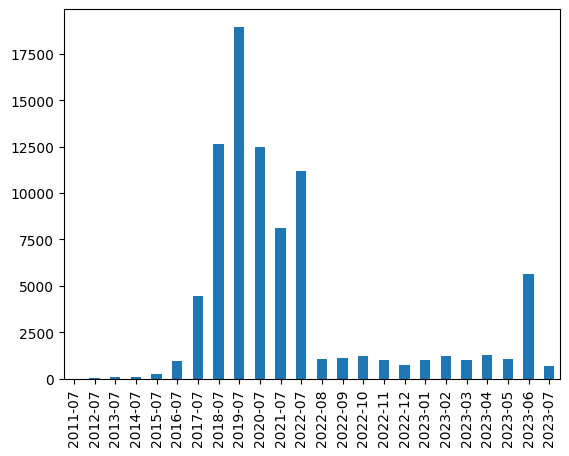
\includegraphics[width=0.75\textwidth]{figs/exploratoria/distribuicao_ano_mes_avaliacao.png}
	\caption{Distribuição do número de avaliação por mês e ano}
	\label{img:dist_ano_mes_avaliacao}
\end{figure}

Agora estamos considerando apenas avaliações que serão utilizadas na analise, a distribuição das notas atribuidas individualmente a cada avaliação pode ser consultada em \ref{img:dist_review_rating}. É fácil notar que grande maioria das avaliações 38347 (77,91\%) foi realizada e atribuida a maior nota, 5, o que nos leva a acreditar que em grande parte o sentimento geral das avaliações é positivo.

\begin{figure}
	\centering
	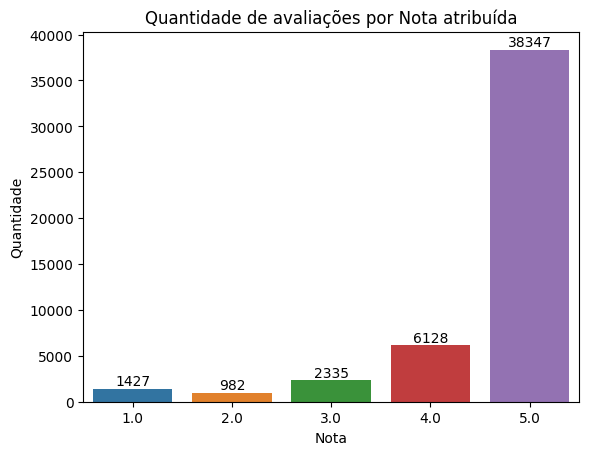
\includegraphics[width=0.75\textwidth]{figs/exploratoria/quantidade_avaliacao_nota_atribuida.png}
	\caption{Quantidade de avaliações por nota atribuida}
	\label{img:dist_review_rating}
\end{figure}

Podemos também observar em \ref{img:dist_review_rating_per_year} a evolução em quantidade númerica durante o tempo, podendo notar uma quebra de tendência no crescimento pós 2019, nos anos de 2020 e 2021, provavelmente causado pelo confinamento decorrente da COVID-21 (referências?) e pós flexibilização do confinamento visualizamos um aumento no número de avaliações, levando em consideração que temos apenas 6 meses de avaliação em 2023 então possivelmente seguiremos com a tendencia de aumento de número de avaliações ano após ano.

Com o grafico \ref{img:relplot_ano_rating} podemos notar que a variação da nota atribuida tende a diminuir conforme o tempo passa, a quantidade de notas maiores é crescente, mas levando em consideração o grafico acima isso talvez seja causado pela crescete também da quantidade de avaliações com notas entre 4 e 5.
\begin{figure}
	\centering
	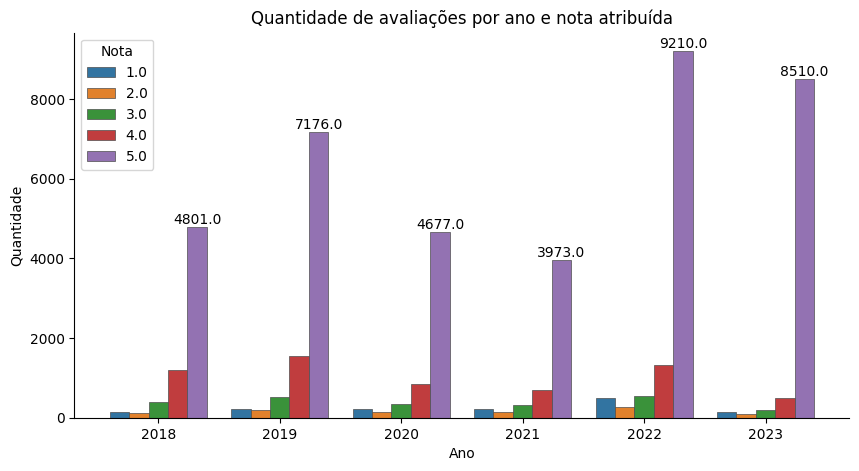
\includegraphics[width=1\textwidth]{figs/exploratoria/quantidade_avaliacao_nota_atribuida_ano.png}
	\caption{Quantidade de avaliações por ano e nota atribuida}
	\label{img:dist_review_rating_per_year}
\end{figure}

\begin{figure}
	\centering
	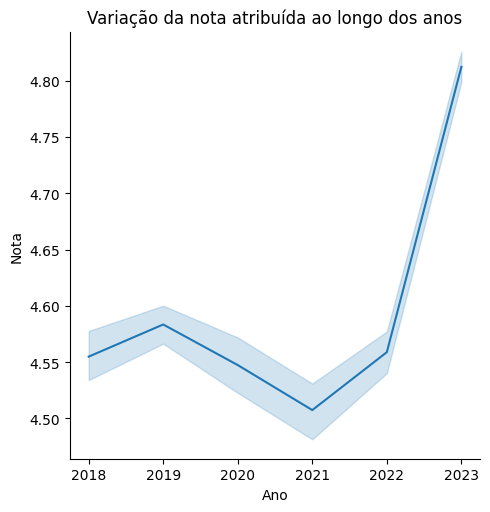
\includegraphics[width=0.70\textwidth]{figs/exploratoria/relplot_ano_rating.png}
	\caption{Variação da nota atribuída ao longo dos anos}
	\label{img:relplot_ano_rating}
\end{figure}

\begin{figure}
	\centering
	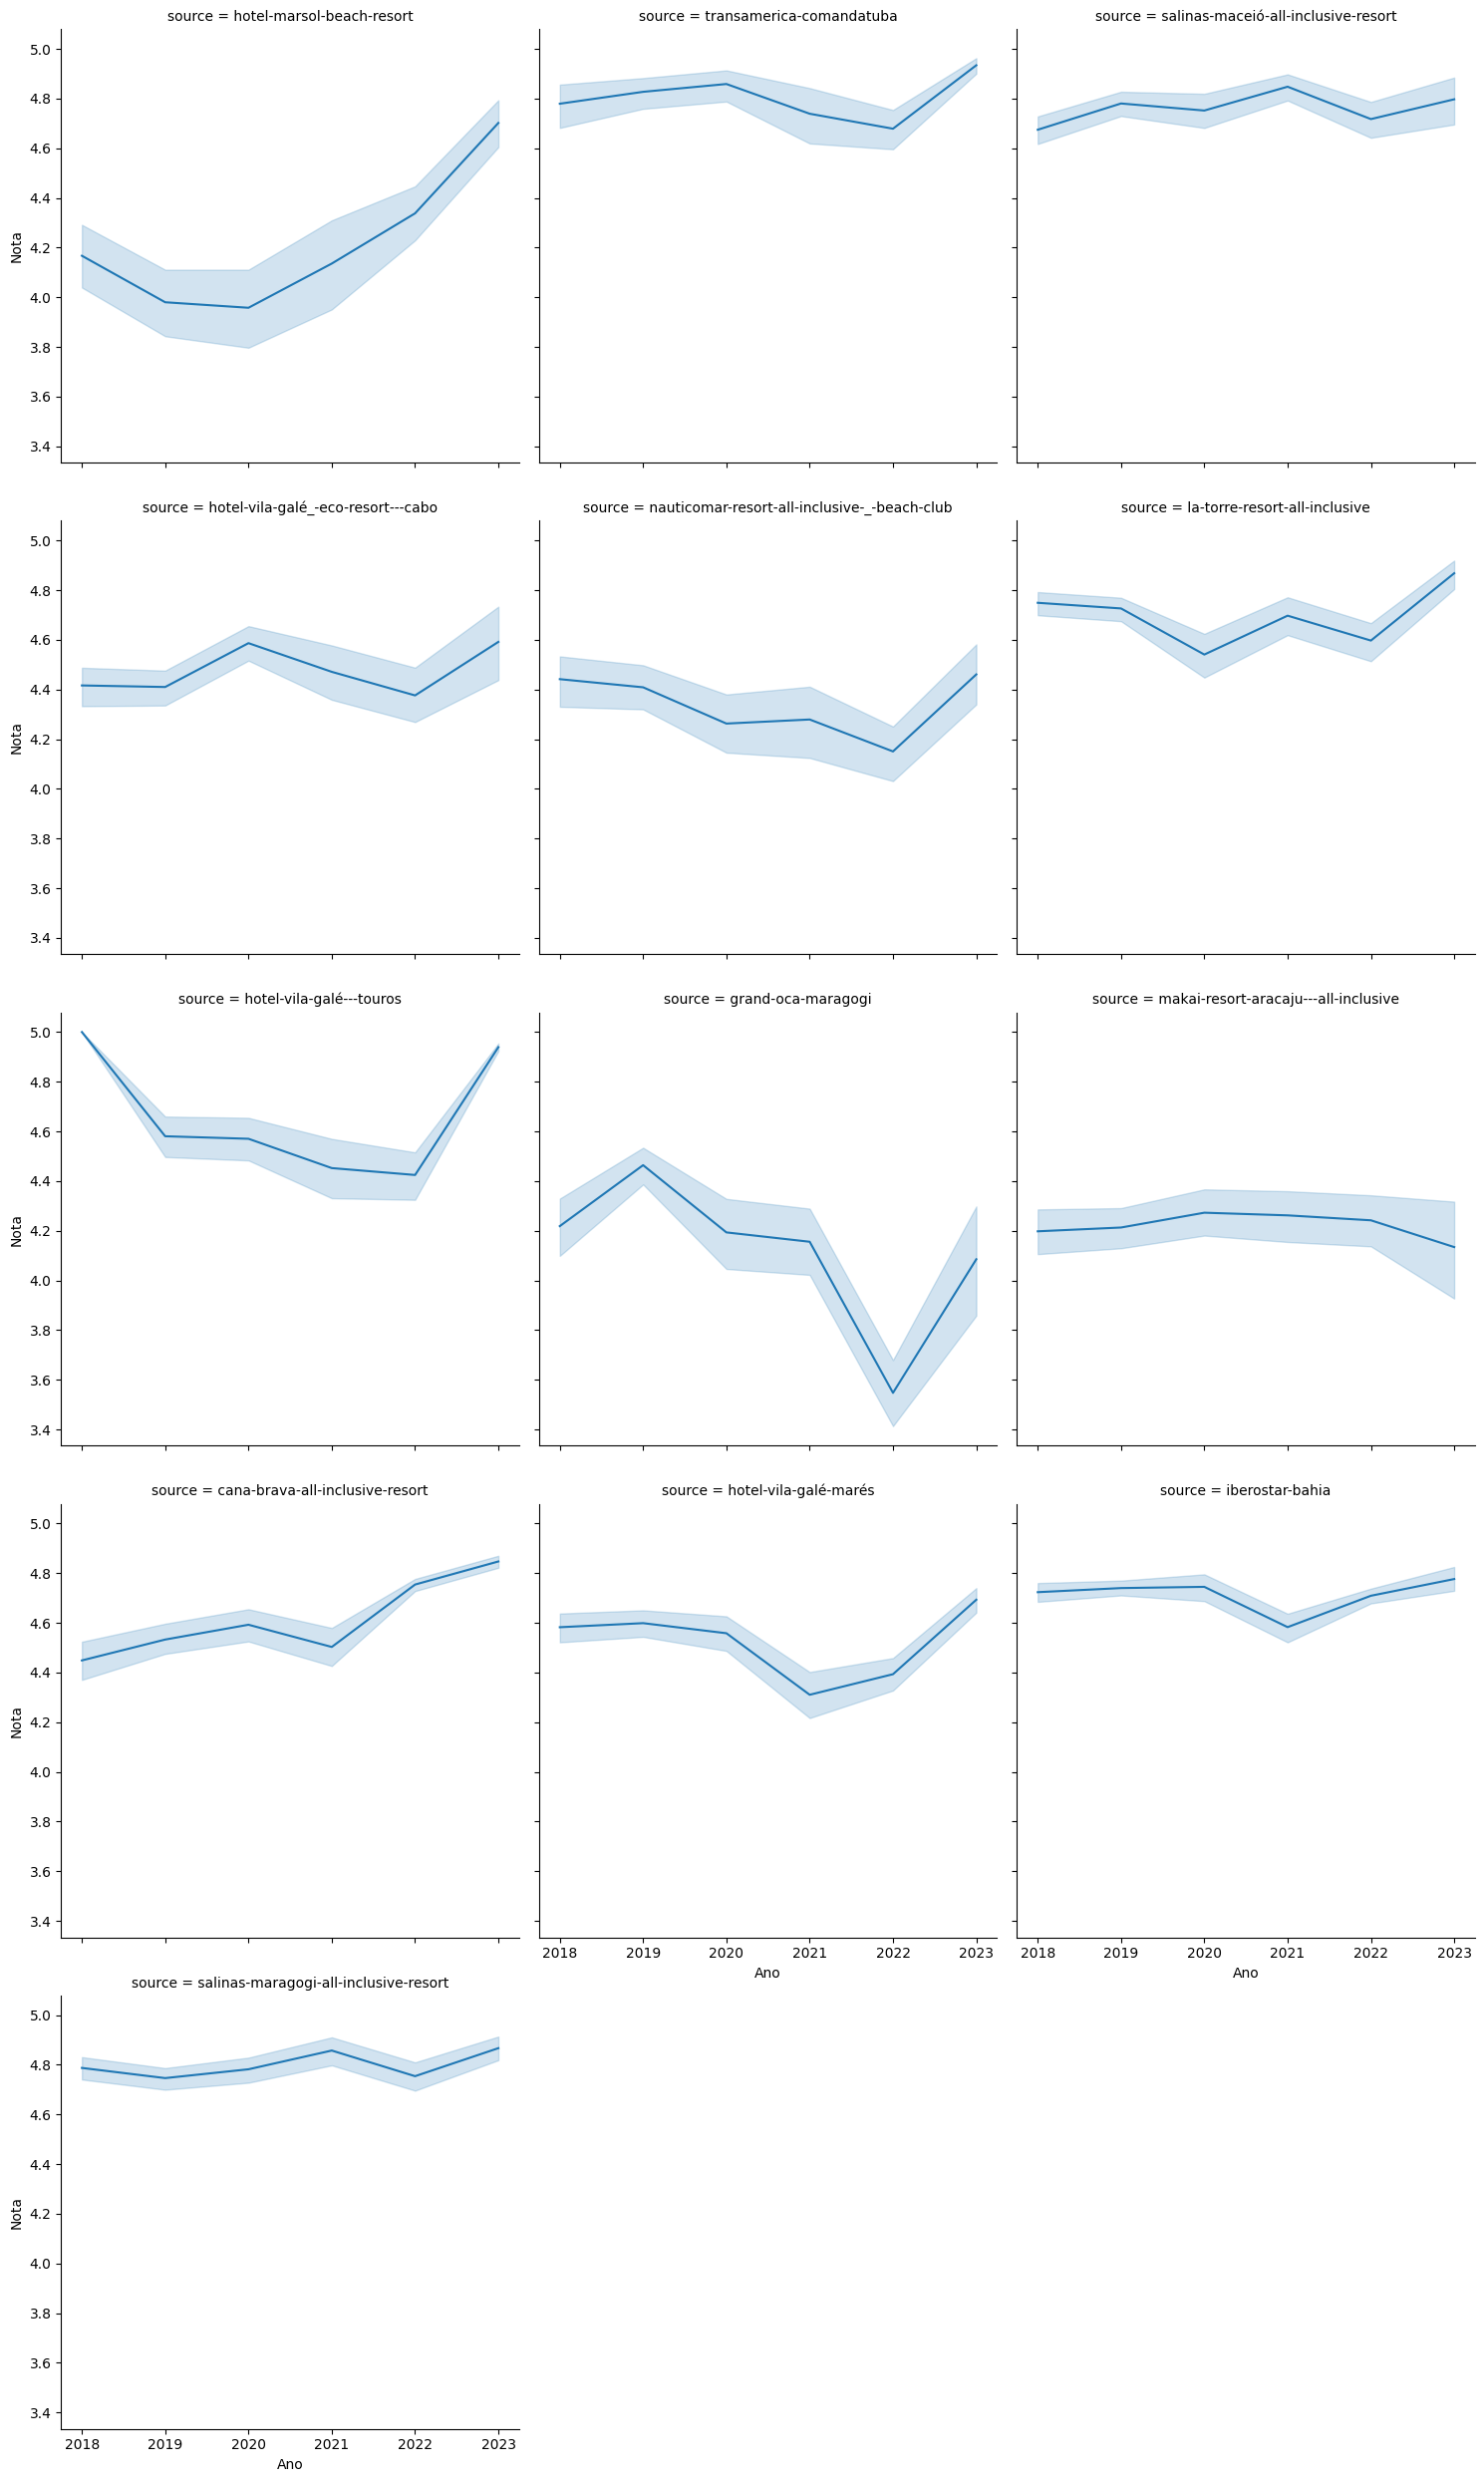
\includegraphics[width=1\textwidth]{figs/exploratoria/relplot_ano_rating_source.png}
	\caption{Variação da nota atribuída ao longo dos anos por hotel}
	\label{img:relplot_ano_rating_source}
\end{figure}


\begin{figure}
	\centering
	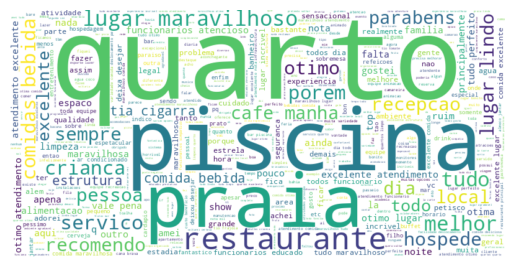
\includegraphics[width=1\textwidth]{figs/exploratoria/wordcloud_geral.png}
	\caption{Wordcloud sem stop words}
	\label{img:wordcloud_geral}
\end{figure}


\begin{figure}
	\centering
	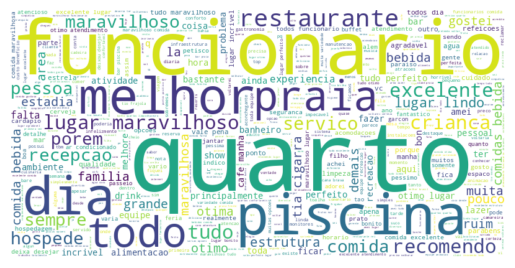
\includegraphics[width=1\textwidth]{figs/exploratoria/wordcloud_substantivos.png}
	\caption{Wordcloud de substantivos}
	\label{img:wordcloud_substantivos}
\end{figure}

\begin{figure}
	\centering
	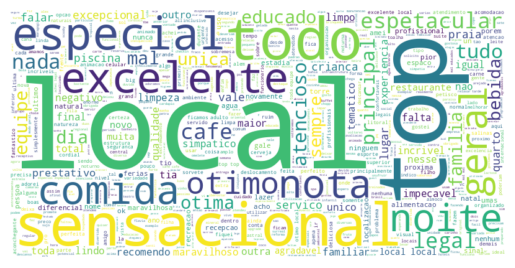
\includegraphics[width=1\textwidth]{figs/exploratoria/wordcloud_adjetivos.png}
	\caption{Wordcloud de Adjetivos}
	\label{img:wordcloud_adjetivos}
\end{figure}

\begin{figure}
	\centering
	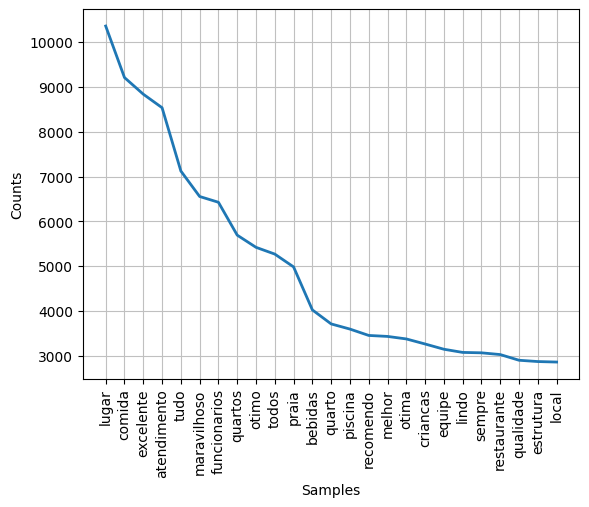
\includegraphics[width=1\textwidth]{figs/exploratoria/unigramas.png}
	\caption{Unigramas}
	\label{img:unigramas}
\end{figure}

\begin{figure}
	\centering
	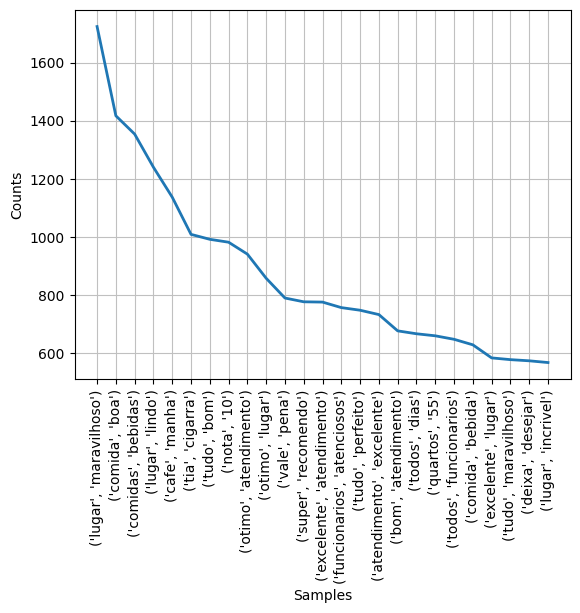
\includegraphics[width=1\textwidth]{figs/exploratoria/bigramas.png}
	\caption{Bigramas}
	\label{img:bigramas}
\end{figure}

\begin{figure}
	\centering
	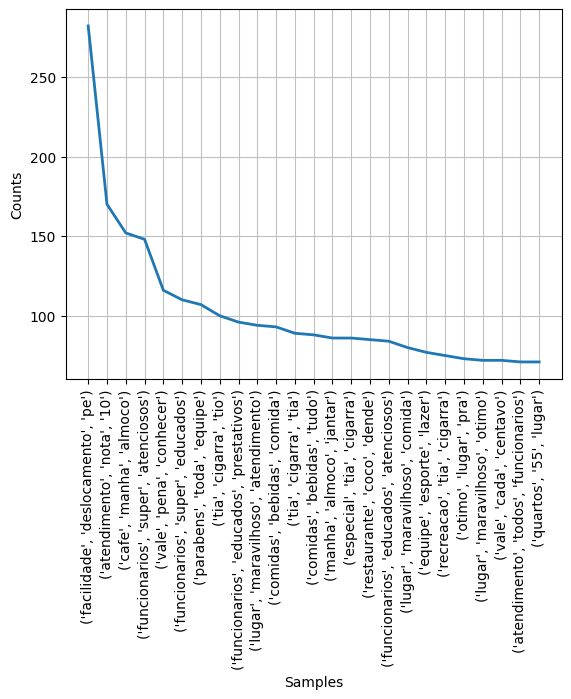
\includegraphics[width=1\textwidth]{figs/exploratoria/trigramas.png}
	\caption{Trigramas}
	\label{img:trigramas}
\end{figure}


%TODO ajustar tamano, ta estranho
\begin{figure}
	\centering
	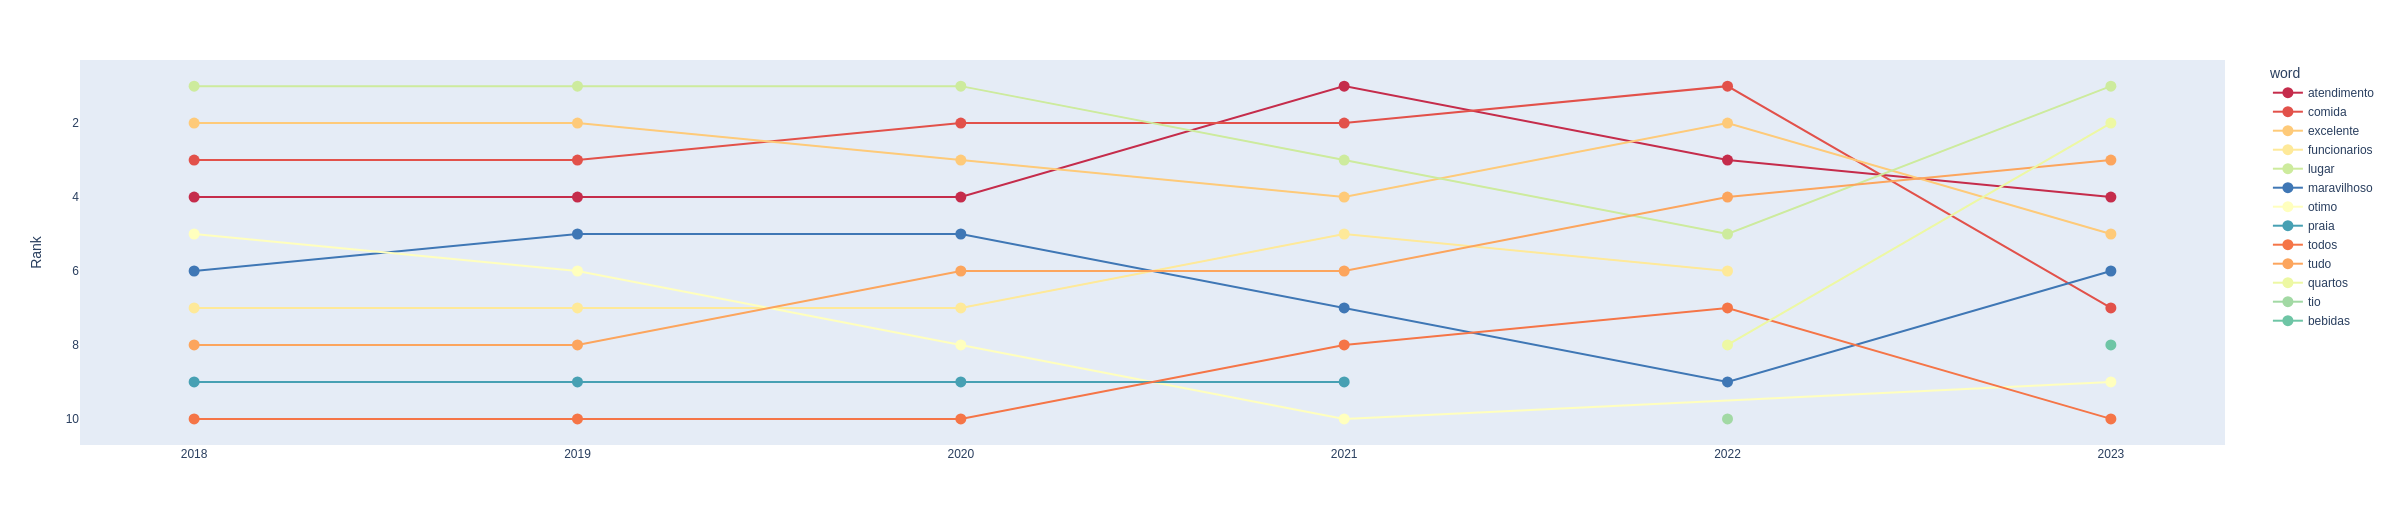
\includegraphics[width=1\textwidth]{figs/exploratoria/ranking_unigramas_por_ano.png}
	\caption{Ranking de unigramas por ano}
	\label{img:rank_unigramas}
\end{figure}


% Please add the following required packages to your document preamble:
% \usepackage{graphicx}
% \usepackage[table,xcdraw]{xcolor}
% Beamer presentation requires \usepackage{colortbl} instead of \usepackage[table,xcdraw]{xcolor}
\begin{table}[]
	\centering
	\begin{tabular}{|p{5cm}|l|l|l|l|}
		\hline
		\textbf{Hotel}                                      &
		\textbf{Não vazio}                                  &
		\textbf{Com texto}                                  &
		\textbf{Traduzido}                                  &
		\textbf{Públicos em +2017}                            \\
		\hline
		\textbf{Cana Brava All Inclusive Resort}            &
		8583                                                &
		8581                                                &
		141                                                 &
		10656                                                 \\
		\hline
		\textbf{Grand Oca Maragogi}                         &
		2948                                                &
		2947                                                &
		542                                                 &
		4297                                                  \\
		\hline
		\textbf{Hotel Marsol Beach Resort}                  &
		2150                                                &
		2150                                                &
		162                                                 &
		3128                                                  \\
		\hline
		\textbf{Hotel Vila Galé - Touros}                   &
		4481                                                &
		4480                                                &
		111                                                 &
		5802                                                  \\
		\hline
		\textbf{Hotel Vila Galé - Marés}                    &
		5723                                                &
		5721                                                &
		315                                                 &
		7981                                                  \\
		\hline
		\textbf{Hotel Vila Galé Eco Resort - Cabo}          &
		3219                                                &
		3217                                                &
		183                                                 &
		4934                                                  \\
		\hline
		\textbf{Iberostar Bahia}                            &
		10587                                               &
		10586                                               &
		1464                                                &
		14848                                                 \\
		\hline
		\textbf{La Torre Resort - All Inclusive}            &
		3847                                                &
		3847                                                &
		496                                                 &
		5722                                                  \\
		\hline
		\textbf{Makai Resort Aracaju - All Inclusive}       &
		3180                                                &
		3180                                                &
		84                                                  &
		4917                                                  \\
		\hline
		\textbf{Nauticomar Resort All Inclusive Beach Club} &
		2630                                                &
		2628                                                &
		228                                                 &
		3938                                                  \\
		\hline
		\textbf{Salinas Maceió All Inclusive Resort}        &
		2836                                                &
		2836                                                &
		168                                                 &
		4497                                                  \\
		\hline
		\textbf{Salinas Maragogi All Inclusive Resort}      &
		4572                                                &
		4572                                                &
		203                                                 &
		6700                                                  \\
		\hline
		\textbf{Transamerica Comandatuba}                   &
		2149                                                &
		2148                                                &
		87                                                  &
		3050                                                  \\ \hline
	\end{tabular}
	\caption{Quantidade de avaliações em cada filtro pro hotél}
	\label{table:qtd_review_filtro}
\end{table}

\begin{table}[]
	\centering
	\begin{tabular}{|l|p{5cm}|p{5cm}|}
		\hline
		\textbf{Campo}            & \textbf{Descrição}                                                              & \textbf{Tipo}                                                                  \\
		\hline
		token                     & token utilizado para buscar a próxima sequencia de avaliações na API            & textual                                                                        \\
		\hline
		review\_id                & identificador da avaliação                                                      & textual                                                                        \\
		\hline
		retrieval\_date           & data na qual o script recuperou a avaliação                                     & textual em formato de datetime                                                 \\
		\hline
		rating                    & valor númerico de nota que foi atribuido ao estabelecimento                     & númerico                                                                       \\
		\hline
		rating\_max               & valor númerico máximo de nota que poderia ter sido atribuido ao estabelecimento & númerico                                                                       \\
		\hline
		relative\_date            & data relativa ao retrieval\_date de quando a avaliação foi públicada            & textual formato de data relativa(1 dia atrás, 1 ano atrás, 3 meses atrás, etc) \\
		\hline
		likes                     & quantidade de Likes que a avaliação recebeu de outros usuários da plataforma    & númerico                                                                       \\
		\hline
		other\_ratings            & avaliações de outros aspectos relacionados ao estabelecimento                   & textual                                                                        \\
		\hline
		trip\_type\_travel\_group & indicador se a viagem foi realizada em grupo                                    & textual                                                                        \\
		\hline
		user\_name                & nome do usuário que realizou a públicação                                       & textual                                                                        \\
		\hline
		user\_is\_local\_guide    & identificador para indicar usuários que são local guides                        & textual                                                                        \\
		\hline
		user\_reviews             & número para indicar a quantidade de avaliações realizardas pelo usuário         & textual                                                                        \\
		\hline
		user\_photos              & número de fotos que o usuário postou                                            & númerico                                                                       \\
		\hline
		user\_url                 & endereço na web do perfil do usuário                                            & textual                                                                        \\
		\hline
		text                      & conteúdo textual da avalição                                                    & textual                                                                        \\
		\hline
		response\_text            & conteúdo textual de uma possivel resposta do estabelecimento à avalição         & textual                                                                        \\
		\hline
		response\_relative\_date  & data relativa ao retrieval\_date de quando a resposta à avaliação foi públicada & string no formato de data relativa                                             \\
		\hline
		errors                    & lista de erros ao tentar fazer o \emph{parse} da avaliação                      & lista textual                                                                  \\
		\hline
	\end{tabular}
	\caption{estrutura da avaliação}
	\label{tab:estrutura_review}
\end{table}

%% BERT
%%
Foram selecionados 5 modelos BERT para serem utilizados, escolhidos com base no ranking disponibilizado pelo hugging faces, sendo eles:
\begin{itemize}
	\item philschmid/distilbert-base-multilingual-cased-sentiment
	\item lxyuan/distilbert-base-multilingual-cased-sentiments-student
	\item citizenlab/twitter-xlm-roberta-base-sentiment-finetunned
	\item cardiffnlp/twitter-xlm-roberta-base-sentiment
	\item ramonmedeiro1/bertimbau-products-reviews-pt-br
\end{itemize}

Todos executados utilizando a biblioteca transformers, utilizando o AutoTokenizer, AutoModelForSequenceClassification e pipeline, executados usando device Cuda(Nvidia RTX 4070TI com 16gb de VRAM) %% mais detalhes do ambiente de execução?

sendo o tempo de execução médio, após 5 execuções cada, para que a analise de todo o corpos fosse realizada, o seguinte:

\begin{itemize}
	\item philschmid/distilbert-base-multilingual-cased-sentiment: 3min e 37s
	\item lxyuan/distilbert-base-multilingual-cased-sentiments-student: 3min e 36s
	\item citizenlab/twitter-xlm-roberta-base-sentiment-finetunned: 6min e 54s
	\item cardiffnlp/twitter-xlm-roberta-base-sentiment: 6min e 44s
	\item ramonmedeiro1/bertimbau-products-reviews-pt-br: 6min e 59s
\end{itemize}

Nessa etapa cada um dos modelos Berts atribuia a avaliação um score indicando a confiança de uma dada label ser a classificação correta daquele review. Após todas as analises terminarem foi realizado então a união dos resultados e a label escolhida será igual a do modelo bert que atribuir o \emph{score} mais alto.


% Nessa etapa utilizaremos o BERT (\emph{Bidirectional Encoder Representations from Transformers}), sendo este um modelo de representação de linguagem desenvolvido por pesquisadores do Google e que teve seu código aberto em 2018~\cite{hugoZanini2021mediu}. O texto será tokenizado utilizando a biblioteca e um modelo pré-treinado denominado "BERTimbau Base"~\cite{souza2020bertimbau}.

% Será realizado também o emparelhamento de Adjetivo-Substantivo visando identificar o sentimento por tópicos contidos na avaliação analisada. Para isso será utilizada a biblioteca spaCy~\cite{montani2022spacy}.

\section{Análise dos dados}

\subsection{Análise de Sentimentos}
\label{subsec:analise_sentimentos}

Com o modelo treinado e os dados prontos para serem classificados, o modelo irá atribuir uma classificação geral para documento, ou seja, cada avaliação individualmente recebera uma classificação do modelo, sendo ela positiva, neutra ou negativa.

\subsection{Análise Temporal}
\label{subsec:analise_temporal}
Após a análise de sentimentos, utilizaremos os resultados agrupados por períodos de modo a conseguir visualizar em modo gráfico as avaliações divididas conforme explicitado na seção anterior para um grupo de hotéis.
